%\chapter{Dataset Analysis and Pre-processing Techniques}
\chapter{Dataset and LIWC}

\label{chap:ch3}

\par
\section{Dataset Overview}

\quad Our AI model relies on a dataset \cite{depressionDataset}, crafted in order to advance in mental health classification research. Gathered through web scraping techniques from diverse Subreddits, this dataset contains discussions and viewpoints on mental health topics. The aim of creating this dataset was to examine textual patterns which indicate depression's presence or absence in individuals, as seen from their online conversations .

% \subsection{Collection Methodology}
The raw data was sourced by employing web scraping techniques, targeting specific Subreddits known for their discussions on mental health issues. This approach ensured that the data collected was relevant to the research objectives, capturing a diverse range of experiences and expressions related to mental health.

% \subsection{Dataset Overview}
Comprising 7,650 unique entries, the dataset is enough for an accurate machine learning algorithm. Each entry is annotated with an is\textunderscore depression label, distinguishing between texts that indicate the presence of depression (labeled '1') and those that do not (labeled '0'). This labeling process was carried out with careful consideration to ensure accuracy and reliability in the classification \cite{depressionDataset}. Examples from the dataset can be seen in Table \ref{datasetEnglishExamples}.

\begin{table}[ht]
\centering
\renewcommand{\arraystretch}{1.5} % Adjust row height
\begin{adjustbox}{width=\textwidth}
\begin{tabular}{|p{0.45\textwidth}|p{0.45\textwidth}|} % Adjust column width
\hline
\textbf{Depression} & \textbf{No Depression} \\ \hline
it s so pointless for me to still be alive my life is worthless why am i still here & this week is not going as i had hoped \\ \hline
i don t know what to feel but i just am tired and over it and there s no end to running on a hamster wheel of constant sadness ugh & i hate when i have to call and wake people up \\ \hline
\end{tabular}
\end{adjustbox}
\caption{Examples of entries in the dataset}
\label{datasetEnglishExamples}
\end{table}


A noteworthy aspect of the dataset is its well-balanced nature, with 3,900 entries labeled as non-depression and 3,831 entries indicating depression. This balance is important in avoiding bias in the predictive modeling process, ensuring that the resulting classification model is accurate.

Also the raw data underwent a cleaning process using multiple Natural Language Processing (NLP) techniques. This pre-processing phase was crucial for eliminating noise, such as irrelevant characters, web links, and non-English words, thereby refining the dataset for analysis. The cleaning process also involved normalizing the text to ensure consistency across the dataset, facilitating more effective data analysis and model training \cite{depressionDataset}.

\subsection{Dataset Translation for Romanian Language}
\par \quad Multilingual depression detection is highly dependant on the capability of AI models to understand and analyze text from different cultures. This section describes the process of translating English text into Romanian, a step essential for training our AI model to recognize depressive patterns in a multilingual context. We will discuss the selection criteria and the impact of utilizing a specific Translation API to bridge the language gap, thus enabling our model to process and interpret Romanian text with the same level of accuracy as English. 

\subsection{Reasoning Behind Choosing Yandex}

\quad In our effort to refine our multilingual depression detection model, we referenced a detailed study that assessed the efficiency, accuracy, and security of various Translation APIs \cite{rashmi2020comparison}. This comparative analysis served as the foundation for selecting the most suitable API for our application, which required the translation of text from English to Romanian among other language pairs. The study meticulously compared several leading Translation APIs, including Google API, Microsoft, Systran.io, MyMemory, and Yandex, focusing on their performance in terms of speed, accuracy, security, and the breadth of language support.
\begin{itemize}
\item \textbf{Google API} is widely recognized for its impressive language support, capable of translating content across more than 100 languages. This extensive reach makes it a versatile tool for global communication and content translation. Its reputation and prevalence in the market are testaments to its utility and user-friendly interface. Additionally, it's worth noting that while Google API is commendable, it is not a free service, which may affect its accessibility for some users.\cite{rashmi2020comparison}.

\item \textbf{Microsoft's Translation API} is lauded for its quality and security, offering translations among 60+ languages. It stands out for its emphasis on accuracy and stringent security protocols, although its language support is less extensive than Google's \cite{rashmi2020comparison}.

\item \textbf{Systran.io} boasts a high accuracy rate of 99\%, albeit with limitations in recognizing slang, nuances, and culturally relevant phrases. Its security is commendable, positioning it as a reliable choice for many applications \cite{rashmi2020comparison}.

\item \textbf{MyMemory} excels in translation speed but experiences the highest latency among the APIs evaluated. While it supports translations between 80+ languages, the absence of training data for certain language combinations limits its effectiveness. Nonetheless, its security is robust \cite{rashmi2020comparison}.

\item \textbf{Yandex API}, with support for 90+ languages, stands out for its balance of translation accuracy and lower latency compared to its counterparts. Despite its efficiency and broad language coverage, its security features are not optimal for translating confidential documents \cite{rashmi2020comparison}.
\end{itemize}

The conclusion from this study discussed the strengths and weaknesses of each API, guiding our choice towards Yandex API for our multilingual depression detection model. Yandex was selected due to its free access, lower latency, and reliable accuracy across different cultures, making it an ideal tool for everyday translations where security is not the biggest concern \cite{rashmi2020comparison}. This choice aligns with our objective of giving people an easy to use and accessible tool in order to prevent problems that could appear with depression.

Another rigorous study \cite{cambedda2021study} provides a nuanced error analysis of Yandex's translations. Notably, Yandex's performance, depicted in the graph \ref{YandexTranslationPerformance}, indicates a relatively uniform distribution of errors across multiple categories. This suggests that while Yandex does have areas where it lacks consitency, such as Lexis, Syntax, and Article Usage, it generally maintains the core meaning of the translated text. This is critical for our model, which relies on emotion categories to accurately detect depression in text.

\begin{figure}[htbp]
	\centering
		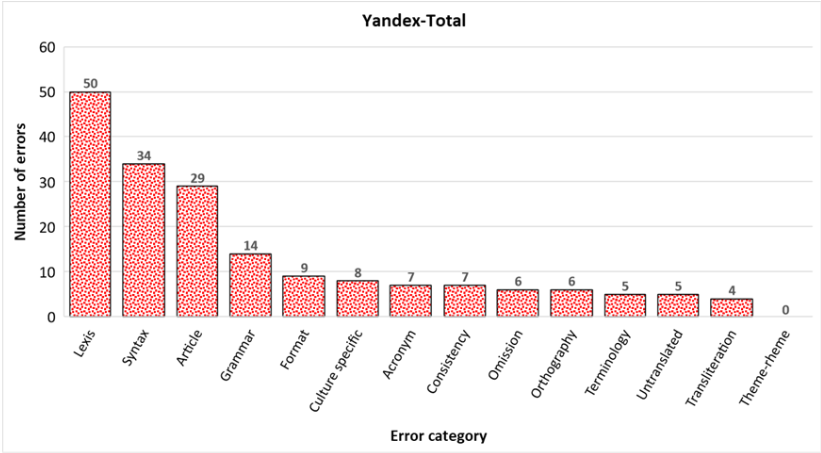
\includegraphics[scale=0.65]{LaTeX Bachelor Thesis Depression Signs Detection/figures/Yandex's-translation-performace.png}
	\caption{Yandex's translation performance \cite{cambedda2021study}}
	\label{YandexTranslationPerformance}
\end{figure}

The Lexis category, in particular, displays the highest number of errors, signaling a need for further investigation to understand whether these issues are from the nature of the texts or from challenges within the translation tool. However, it is encouraging to note that error categories such as Grammar, Format, Culture-Specific References, Acronym, and Consistency show significantly fewer errors. These categories are essential for maintaining the general meaning, which reaffirms our choice of Yandex for texts where nuanced meaning is less likely to affect the detection of depression signs.

Further examination of the study indicates that Yandex demonstrates a more adept handling of common language texts as opposed to those with specialized jargon, registering fewer errors in translations of texts with language spoken by the people in a particular country or region \cite{cambedda2021study}. Considering our dataset comprises of Reddit posts, which are typically phrased in everyday language, this finding is particularly relevant. The study also highlights that, with the exception of Article Usage, the disparity in error rates between different text types is negligible, suggesting that Yandex can reliably manage the conversational and informal style characteristic of Reddit communications.

\subsection{Adjusting to Yandex API's Policy Shift}

\quad We had initially recognized the Yandex API as a superior option, particularly for its cost-effectiveness, as it was freely accessible at the time of study \cite{rashmi2020comparison}. This advantage aligned with our objectives, allowing us to use its translation capabilities without financial constraints.

However, since the publication of \cite{rashmi2020comparison}, Yandex's policy has undergone significant changes. The API, once free to use within a given generous limit, now requires users to possess a registered and legally recognized company to utilize its services. Ihe requirement of company registration introduces a barrier, limiting the accessibility of Yandex API for independent researchers, small teams, or educational institutions.

Given these new rules, we are still fully dedicated to creating a useful and easy-to-use depression detection system that works in many languages. Therefore, we are looking into different approaches.

\subsection{Shifting to googletrans}

\quad We decided to integrate the googletrans library \cite{googletranslib} into our multilingual depression detection model. It offers a free and unlimited Python library that uses the Google Translate API. This library appears particularly advantageous for our requirements, as it is not only accessible without cost but also does not require the a company registration that Yandex now demands. As it can be seen in \ref{codeGoogleTransUsage}, it is very accessible to translate text in Python from English ro Romanian.

\begin{figure}[htbp]
	\centering
		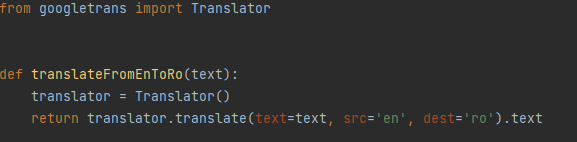
\includegraphics[scale=1]{LaTeX Bachelor Thesis Depression Signs Detection/figures/codeGoogleTransUsage.png}
	\caption{Python library "googletrans" translation from English to Romanian}
	\label{codeGoogleTransUsage}
\end{figure}

The googletrans library \cite{googletranslib} has features that are well-suited to our project's needs. It is recognized for its speed and reliability, as it operates on the same servers as translate.google.com. The library supports auto language detection, facilitating the identification and translation of a wide array of languages without prior specification. Additionally, it provides the capability for bulk translations, which is invaluable when processing large datasets typically found in NLP tasks. It was done for the chosen dataset \cite{depressionDataset} in Python as it can be seen in \ref{codeDatasetTranslation} .

\begin{figure}[htbp]
	\centering
		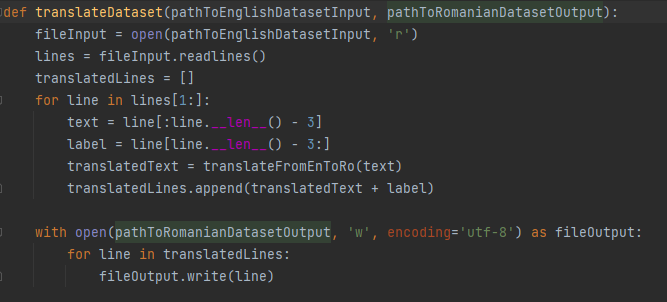
\includegraphics[scale=1]{LaTeX Bachelor Thesis Depression Signs Detection/figures/codeDatasetTranslation.png}
	\caption{Python code for translating dataset from English to Romanian}
	\label{codeDatasetTranslation}
\end{figure}

It is also important to acknowledge googletrans's \cite{googletranslib} usage notes. The 15,000-character limit per text may require segmentation of longer entries, and the instability of web-based translation services means that we should proceed with precaution regarding the library's reliability. The developers themselves suggest opting for the official Google Translate API for more advanced applications where stability is very important. Furthermore, potential HTTP errors could indicate temporary bans by Google, meaning that it is needed to keep an eye on and manage how we use our API to avoid any interruptions. Despite these considerations, the googletrans library's free and flexible usage makes it an excellent fit for our project in its current stage. The examples presented in the original dataset, shown in table \ref{datasetEnglishExamples}, can be seen translated in table \ref{datasetRomanianExamples}.

\begin{table}[ht]
\centering
\renewcommand{\arraystretch}{1.5} % Adjust row height
\begin{adjustbox}{width=\textwidth}
\begin{tabular}{|p{0.45\textwidth}|p{0.45\textwidth}|} % Adjust column width
\hline
\textbf{Depression} & \textbf{No Depression} \\ \hline
Este atât de inutil să fiu încă în viață viața mea este inutilă de ce sunt încă aici. & Săptămâna aceasta nu va merge așa cum am sperat.\\ \hline
Nu știu ce să simt dar sunt doar obosit și peste asta și nu se termină să alerg pe o roată de hamster de tristețe constantă. & Urăsc când trebuie să sun și să trezesc oamenii. \\ \hline
\end{tabular}
\end{adjustbox}
\caption{Examples of entries in the Romanian dataset}
\label{datasetRomanianExamples}
\end{table}


\section{Leveraging LIWC for Textual Analysis}

\quad In natural language processing, especially within the context of psychological research, the tool we choose to process and interpret the data is as important as the data itself. For this reason, our exploration of the dataset uses a text analysis software, namely LIWC (Linguistic Inquiry and Word Count).

In this section, we will explore the specific features of LIWC that make it an invaluable tool for our research purposes. 


\subsection{The Evolution of LIWC}

\quad The Linguistic Inquiry and Word Count (LIWC) tool is a solution for processing and analyzing textual data within the domain of psychological research. This software, coupled with its comprehensive dictionary, bridges the gap between linguistic constructs and psychological theories, offering insights into the dimensions of language.

\quad The LIWC-22 Dictionary is the last iteration of the software, embodying the fusion of linguistic constructs with psychosocial theories through an extensive lexicon. This core component, comprising over 12,000 words, word stems, phrases, and select emoticons, is organized into categories and subcategories designed to capture a wide array of feelings. This arrangement allows for a accurate analysis of text, offering insights into the psychological state, social relationships, and cognitive processes of individuals based on their word usage.

The LIWC-22 Dictionary has a hierarchical organization, where words are not only categorized but also interlinked across multiple dimensions. For instance, the word "cried" contributes to categories such as emotion and sadness, illustrating the dictionary's complexity and depth. This structure enables LIWC-22 to provide a comprehensive analysis of text, reflecting various emotional and cognitive dimensions \cite{boyd2022development}.

In the table \ref{examplesLIWC22Dic} there are examples of the words linked to their coresssponding categories and it can be seen that the words represent specifics of their category. 

\begin{table}[ht]
\centering
\begin{tabular}{llll}
\hline
\textbf{Social} & \textbf{Culture} & \textbf{Lifestyle} & \textbf{Physical} \\ \hline
admiration & norwegian & free time & abs \\
company & nuclear & accomplish & aerobic\\
listener & online & real estate & ailment\\
locals & arabic & gaming & alcohol\\
refugee & political & qualify & deaf\\
reassure & phonecall & amusement &  death\\
trust & person of color & god &  kidney\\
tweets & racist &  remodel &  lactose\\
twins & bill of rights & art & salad\\
uncle & scanner & greed & ketogen\\
loyal & bots & rent &  depressed\\
commitment & candidate & assignment &  diabet\\
confess & opposition party & psychologist & sauna\\ \hline
\end{tabular}
\caption{Examples of categories and its words in LIWC-22}
\label{examplesLIWC22Dic}
\end{table}


The development of the LIWC-22 Dictionary represents a significant evolution from its predecessors, incorporating advances in computational linguistics and psychological research. The creation process involved multiple phases:
\begin{itemize}
\item Word Collection: Leveraging the foundation of the LIWC2015 dictionary, new words were generated for each category through a combination of expert input and comprehensive literature review \cite{boyd2022development}.
\item Judge Rating Phase: Words were qualitatively assessed by a panel of judges for their fit within each category, with disagreements resolved through in-depth analysis and consensus.
Base Rate Analyses: Utilizing the Meaning Extraction Helper (MEH) tool, the frequency of dictionary words in a diverse corpus was evaluated to ensure relevance and applicability across various text samples \cite{boyd2022development}.
\item Candidate Word List Generation: Through statistical analysis and expert review, candidate words were identified for potential inclusion in the dictionary, ensuring a broad and relevant lexicon \cite{boyd2022development}.
\item Psychometric Evaluation: Each category underwent rigorous testing for internal consistency, with adjustments made to optimize the dictionary's psychometric properties \cite{boyd2022development}.
\item Refinement Phase: The entire process was iteratively refined to address any oversights and enhance the dictionary's accuracy and reliability \cite{boyd2022development}.
\item Addition of Summary Variables: New summary variables were introduced to provide additional analytical dimensions, based on cutting-edge research \cite{boyd2022development}.
\end{itemize}

The LIWC-22 Dictionary has been significantly expanded to include not only traditional words but also numbers, punctuation, short phrases, and regular expressions. This expansion allows for the analysis of modern, informal communication styles found on social media and text messaging, incorporating "netspeak" and emoticons for a more comprehensive understanding of digital communication. All features used in processing the dataset can be seen in Figures \ref{LIWC22EnglishDicF1} and \ref{LIWC22EnglishDicF2}.

\begin{figure}[htbp]
	\centering
		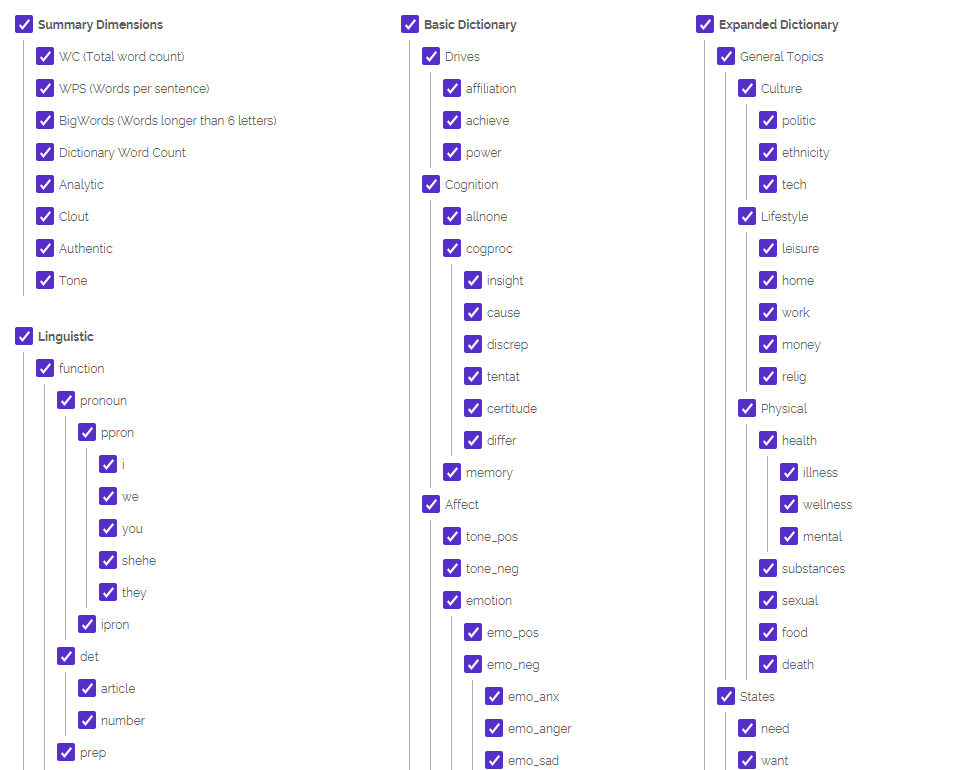
\includegraphics[scale=0.5]{./figures/LIWC22EnglishFeatures1.png}
	\caption{LIWC-22 English Dictionary Features First Part }
	\label{LIWC22EnglishDicF1}
\end{figure}

\begin{figure}[htbp]
	\centering
		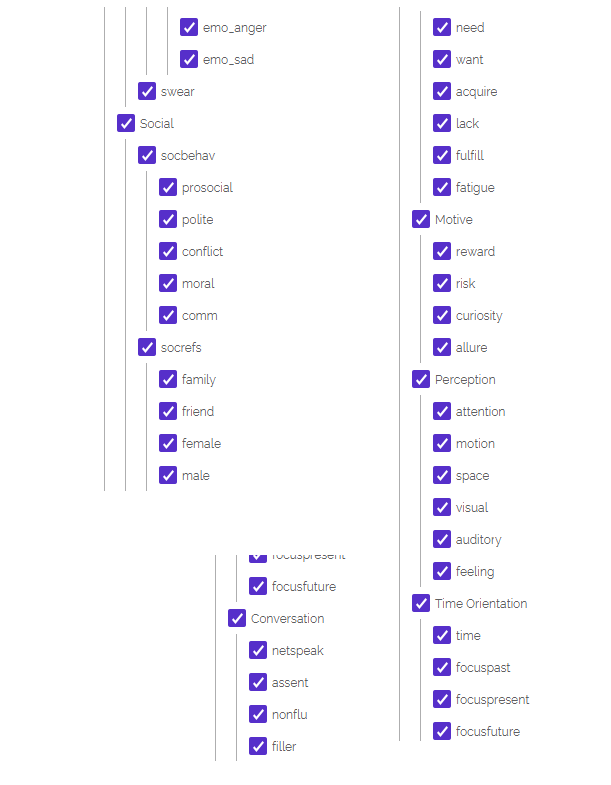
\includegraphics[scale=0.65]{./figures/LIWC22EnglishFeatures2.png}
	\caption{LIWC-22 English Dictionary Features Second Part }
	\label{LIWC22EnglishDicF2}
\end{figure}



The dictionary's evolution reflects a balance between expert human judgment and sophisticated computational models, ensuring that LIWC-22 remains at the forefront of text analysis technology. With each iteration, LIWC has adapted to the changing landscape of language use, incorporating new categories and adjusting existing ones to better capture the psychological significance of language \cite{boyd2022development}. However, the most recent English dictionary for LIWC-22 has not been translated into Romanian. The latest available version for Romanian is the LIWC-2015 dictionary, which contains only 86 features, compared to the 119 features available in the English version. This dictionary was used for processing the translated dataset into Romanian and its features can be seen in Figures \ref{LIWC2015RomanianDicF1} and \ref{LIWC2015RomanianDicF2}.


\begin{figure}[htbp]
	\centering
		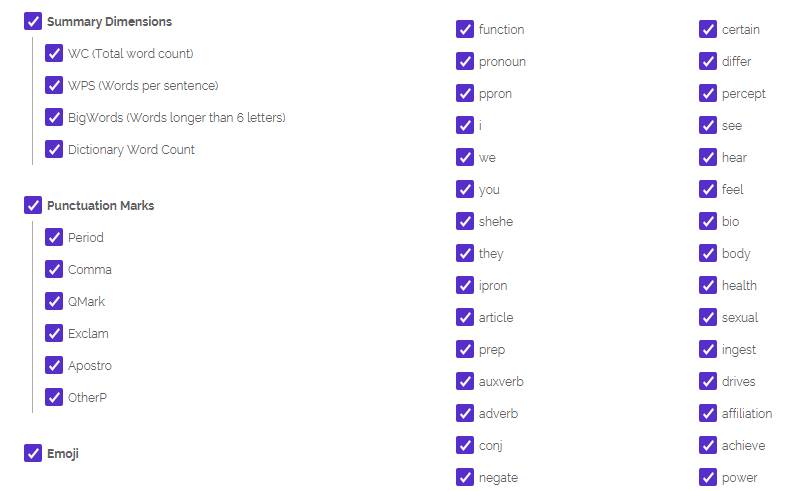
\includegraphics[scale=0.65]{./figures/LIWC2015RomanianFeatures1.png}
	\caption{LIWC-2015 Romanian Dictionary Features First Part }
	\label{LIWC2015RomanianDicF1}
\end{figure}


\begin{figure}[htbp]
	\centering
		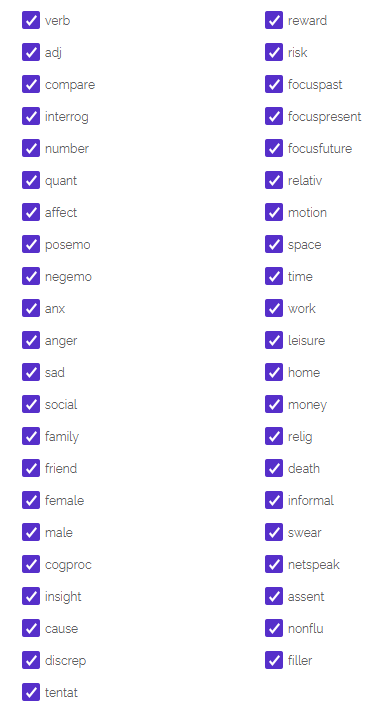
\includegraphics[scale=0.65]{./figures/LIWC2015RomanianFeatures2.png}
	\caption{LIWC-2015 Romanian Dictionary Features Second Part }
	\label{LIWC2015RomanianDicF2}
\end{figure}

\subsection{The Reliability of LIWC}

\quad The development of the Linguistic Inquiry and Word Count (LIWC-22) tool has consistently prioritized the establishment of a scientifically accurate system, focusing on both reliability and validity. This commitment has guided each iteration of LIWC, with the aim of adapting to the dynamic nature of language use and leveraging the research of text-based data science. LIWC-22 represents the culmination of these efforts, integrating dictionaries with cutting-edge data analytics to offer a highly validated tool for text analysis.

The core of LIWC-22's reliability lies in the "Test Kitchen" corpus [Figure \ref{FigKitchenCorpus}], a carefully chosen set of English language examples taken from many different places. This corpus serves two purposes: it is important in the selection of words for the LIWC-22 dictionary and plays a crucial role in assessing the dictionary's reliability and validity. The diversity of the Test Kitchen corpus [Figure \ref{FigKitchenCorpus}] ensure that LIWC-22's analyses are grounded in a realistic representation of language used across various contexts \cite{boyd2022development}.

The Test Kitchen corpus [Figure \ref{FigKitchenCorpus}] was assembled from 15 distinct English language data sets, encompassing a wide range of communication forms, from blogs and emails to social media posts and movie dialogues. This corpus consists of 15,000 texts, with each text sample reflecting the unique linguistic style of its author or authors. The selection process for these samples was designed to include a diverse representation of texts, ensuring a broad coverage of language use in daily life. 

In Figure \ref{FigKitchenCorpus} Word Count M represents the average number of words in the texts for each type of document. For example, the average word count for applications is 1506 words. SD is the standard deviation and this measures how spread out the word counts are around the average. A small SD means the word counts are close to the average, while a large SD means they vary more. For example, in applications, the SD of 501 means most essays have word counts close to 1506, but they can differ by about 501 words.

The construction of this corpus involved selecting 1,000 text samples from each of the 15 sources, with each text containing at least 100 words. For longer texts, a specific algorithm was employed to extract a continuous segment of 10,000 words, ensuring a manageable and consistent analysis size. In total, the Test Kitchen corpus [Figure \ref{FigKitchenCorpus}] encompasses over 31 million words, providing a good foundation for the validation and refinement of the LIWC-22 dictionary \cite{boyd2022development}.

Given the sensitivity and proprietary nature of some of the data sources, the Test Kitchen corpus, while invaluable for the development and testing of LIWC-22, cannot be made publicly available. This restriction shows the careful consideration given to privacy and ethical research practices in the compilation and use of the corpus. Nevertheless, the corpus's diverse and extensive dataset has been crucial in fine-tuning LIWC-22's dictionaries to reflect genuine language usage patterns .

\begin{figure}[htbp]
	\centering
		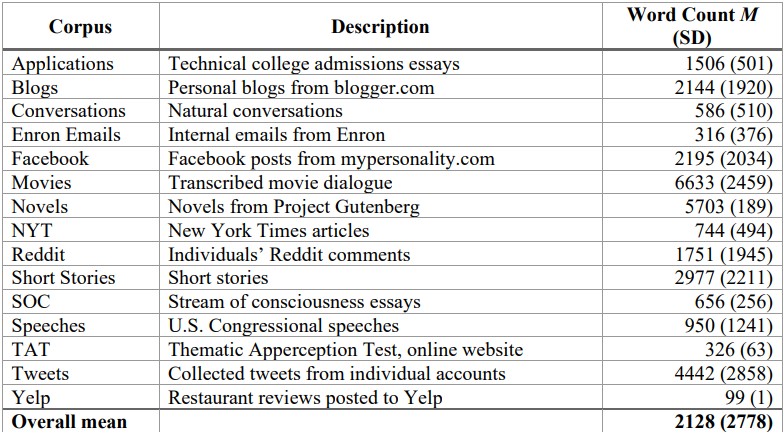
\includegraphics[scale=0.65]{./figures/test-kitchen-corpus.png}
	\caption{The Test Kitchen Corpus of 31 Million Words \cite{boyd2022development}}
	\label{FigKitchenCorpus}
\end{figure}

Quantifying the reliability and validity of text analysis tools like LIWC-22 presents challenges different from traditional psychological assessments. Unlike structured questionnaires, natural language doesn't follow repetitive patterns, making it necessary to adjust standards for language-based analyses. This is due to the dynamic nature of verbal behavior in real-world communication, such as social media posts or conversations, where thoughts are expressed and then move on to the next topic.

Evaluating LIWC-22's reliability involves adapting to this non-repetitive nature. For example, the LIWC-22 Anger scale includes 181 words and phrases related to anger. The use of one anger-related word should theoretically correlate with others in the same text. By analyzing these correlations across various texts, LIWC-22 determines internal consistency \cite{boyd2022development}. Validating LIWC's dimensions is complex. While the categories appear relevant, it's crucial to understand how personal and social psychological processes are reflected in language use. For instance, frequent use of words related to "affiliation" may indicate social connections and needs. Determining whether such language use offers insights into someone's social relationships is vital.

LIWC-22 uses Cronbach’s alpha for continuous data and the Kuder–Richardson Formula 20 (KR-20) for binary data to compute reliability metrics \cite{kuder1937theory}. Traditional methods may underestimate reliability due to variable word usage rates. KR-20, however, provides a more accurate measure by considering the binary nature of word presence.

In 2021, over 2,400 studies used LIWC to examine text, combining text analysis with social and psychological behaviors. These studies, including those from LIWC's developers, found correlations between text-detected emotions and self-reported feelings, showing the tool's capability to capture psychological dynamics. Higher correlations were observed when comparing judges' ratings of writing samples with LIWC scores, indicating consistent external validation \cite{boyd2022development}.